\section{Troubleshooting}\label{troubleshooting}

\subsection{StarRiver Server service fails to start under Windows
XP}\label{starriver-server-service-fails-to-start-under-windows-xp}

A possible cause is that Windows has reached its log size limit. Here is
a solution.

\begin{enumerate}
\def\labelenumi{\arabic{enumi}.}
\itemsep1pt\parskip0pt\parsep0pt
\item
  Open \textbf{Control Panel}. Click \textbf{Performance and
  Maintenance}, then click \textbf{Administrative Tools}, then double
  click \textbf{Event Viewer}.
\item
  Right click \textbf{Application} under \textbf{Event Viewer (Local)},
  then select \textbf{Properties}. 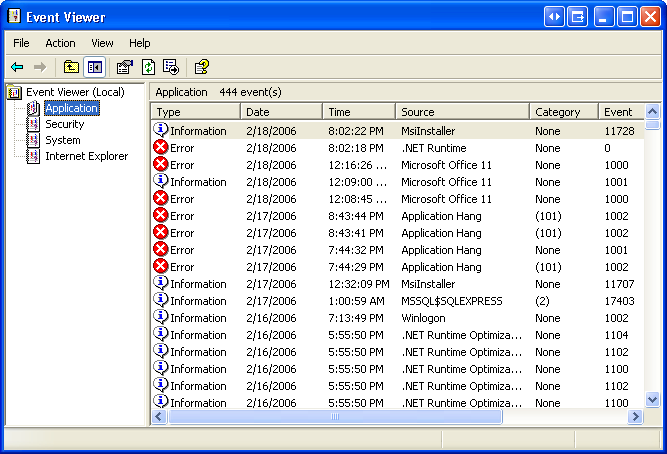
\includegraphics{img/winxp_event.png}
\item
  In \textbf{Application Properties}, inside the \textbf{Log size} box,
  select \textbf{Overwrite events as needed}, then click \textbf{OK}.
  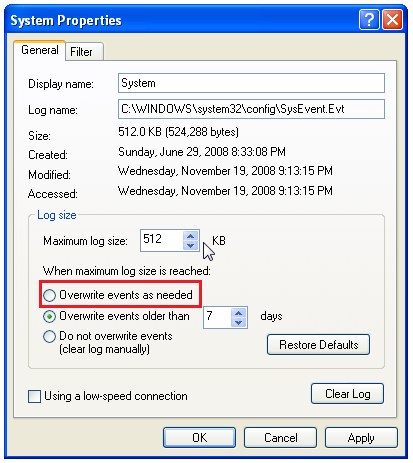
\includegraphics{img/winxp_event_overwrite.png}
\item
  Repeat step 2 and 3 on \textbf{System} under \textbf{Event Viewer
  (Local)}.
\end{enumerate}
